
%(BEGIN_QUESTION)
% Copyright 2010, Tony R. Kuphaldt, released under the Creative Commons Attribution License (v 1.0)
% This means you may do almost anything with this work of mine, so long as you give me proper credit

Dette er en elektronisk varmeledningsevnesensor, brukt til å detektere ulike kjemiske komponenter som kommer ut av kolonnen i en kromatograf. Både måle- og referansefilament varmes av strømmen som går gjennom dem, og det utvikles en varierende spenning over hver av dem når de kjøles ulikt av gassene:

$$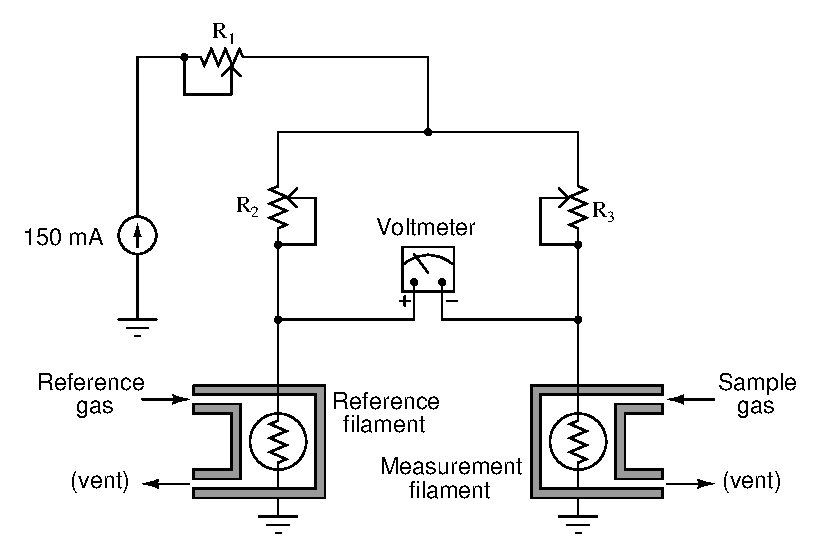
\includegraphics[width=15.5cm]{i00909x01.eps}$$

Anta at en tekniker setter opp detektoren for aller første gang, og ser at voltmeteret viser et unormalt stort signal (med vist polaritet) selv om samme testgass sendes gjennom begge celler.

Vurder sannsynligheten for hver angitt feil i denne kretsen. Se på én feil om gangen (dvs. ingen samtidige feil), og avgjør om feilen alene kan forklare {\it alle} målinger og symptomer i kretsen.

% No blank lines allowed between lines of an \halign structure!
% I use comments (%) instead, so that TeX doesn't choke.

$$\vbox{\offinterlineskip
\halign{\strut
\vrule \quad\hfil # \ \hfil & 
\vrule \quad\hfil # \ \hfil & 
\vrule \quad\hfil # \ \hfil \vrule \cr
\noalign{\hrule}
%
% First row
{\bf Feil} & {\bf Mulig} & {\bf Umulig} \cr
%
\noalign{\hrule}
%
% Another row
$R_1$ motstand satt for lavt &  &  \cr
%
\noalign{\hrule}
%
% Another row
$R_1$ motstand satt for høyt &  &  \cr
%
\noalign{\hrule}
%
% Another row
$R_2$ motstand satt for lavt &  &  \cr
%
\noalign{\hrule}
%
% Another row
$R_2$ motstand satt for høyt &  &  \cr
%
\noalign{\hrule}
%
% Another row
$R_3$ motstand satt for lavt &  &  \cr
%
\noalign{\hrule}
%
% Another row
$R_3$ motstand satt for høyt &  &  \cr
%
\noalign{\hrule}
%
% Another row
Referansefilament brent av (åpen) &  &  \cr
%
\noalign{\hrule}
%
% Another row
Målefilament brent av (åpen) &  &  \cr
%
\noalign{\hrule}
%
% Another row
Voltmeter har feilet åpen &  &  \cr
%
\noalign{\hrule}
%
% Another row
Voltmeter har feilet kortsluttet &  &  \cr
%
\noalign{\hrule}
} % End of \halign 
}$$ % End of \vbox


\underbar{file i00909}
%(END_QUESTION)





%(BEGIN_ANSWER)

% No blank lines allowed between lines of an \halign structure!
% I use comments (%) instead, so that TeX doesn't choke.

$$\vbox{\offinterlineskip
\halign{\strut
\vrule \quad\hfil # \ \hfil & 
\vrule \quad\hfil # \ \hfil & 
\vrule \quad\hfil # \ \hfil \vrule \cr
\noalign{\hrule}
%
% First row
{\bf Feil} & {\bf Mulig} & {\bf Umulig} \cr
%
\noalign{\hrule}
%
% Another row
$R_1$ motstand satt for lavt &  & $\surd$ \cr
%
\noalign{\hrule}
%
% Another row
$R_1$ motstand satt for høyt &  & $\surd$ \cr
%
\noalign{\hrule}
%
% Another row
$R_2$ motstand satt for lavt & $\surd$ &  \cr
%
\noalign{\hrule}
%
% Another row
$R_2$ motstand satt for høyt &  & $\surd$ \cr
%
\noalign{\hrule}
%
% Another row
$R_3$ motstand satt for lavt &  & $\surd$ \cr
%
\noalign{\hrule}
%
% Another row
$R_3$ motstand satt for høyt & $\surd$ &  \cr
%
\noalign{\hrule}
%
% Another row
Referansefilament brent av (åpen) & $\surd$ &  \cr
%
\noalign{\hrule}
%
% Another row
Målefilament brent av (åpen) &  & $\surd$ \cr
%
\noalign{\hrule}
%
% Another row
Voltmeter har feilet åpen &  & $\surd$ \cr
%
\noalign{\hrule}
%
% Another row
Voltmeter har feilet kortsluttet &  & $\surd$ \cr
%
\noalign{\hrule}
} % End of \halign 
}$$ % End of \vbox


%(END_ANSWER)





%(BEGIN_NOTES)

$$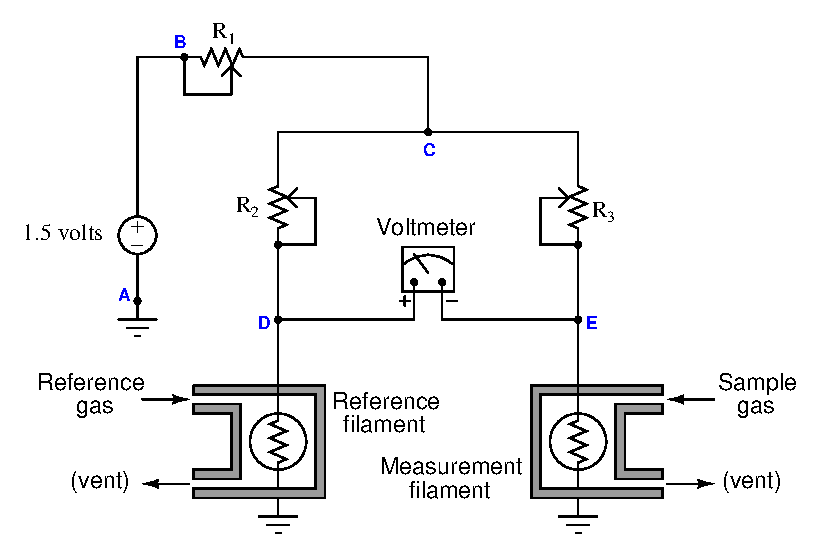
\includegraphics[width=15.5cm]{i00909x02.eps}$$

\vskip 20pt \vbox{\hrule \hbox{\strut \vrule{} {\bf Virtuell feilsøking} \vrule} \hrule}

Denne oppgaven egner seg godt som en ``virtuell feilsøkings''-øvelse. Når du presenterer diagrammet for studentene, forestiller du deg først en bestemt feil i systemet. Deretter presenterer du ett eller flere symptomer på denne feilen (noe som kan observeres av en operatør eller annen bruker). Studentene foreslår så ulike diagnostiske tester for å identifisere feilens art og plassering, som om de var teknikere som feilsøker problemet. Din jobb er å fortelle hva resultatet blir for hver foreslåtte test, og dokumentere resultatene slik at alle studentene ser dem.

Under og etter øvelsen er det nyttig å stille oppfølgingsspørsmål som:

\begin{itemize}
\item{} Hva forteller resultatet av den siste diagnostiske testen om feilen?
\item{} Anta at resultatet av den siste diagnostiske testen hadde vært annerledes. Hva ville det da fortalt om feilen?
\item{} Er den siste diagnostiske testen den beste testen vi kunne gjort?
\item{} Hva ville vært ideell testrekkefølge for å diagnostisere problemet med færrest mulig trinn?
\end{itemize}


%INDEX% Measurement, analytical: chromatography
%INDEX% Troubleshooting review: electric circuits

%(END_NOTES)

